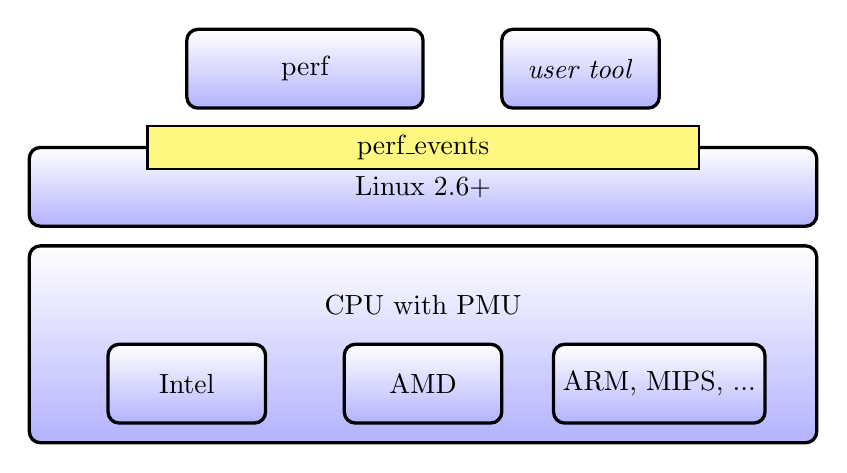
\begin{tikzpicture}[scale=1,transform shape]
\tikzstyle{size}=[minimum width=2 cm, minimum height=1 cm,anchor=center]

\tikzstyle{module}=[size,rectangle,rounded corners,draw=black, top color=white, bottom color=blue!30,very thick, text centered]
\tikzstyle{interface}=[rectangle,draw=black, fill=yellow!50,thick, text centered]
\tikzstyle{label}=[size,rectangle,text centered]

\node [module,minimum width=10 cm,minimum height=2.5 cm] at (0,0.5) (cpu)  {};
\node [label] at (0,1) (cpuLabel) {CPU with PMU};
\node [module] at (-3,0) (intel)  {Intel};
\node [module] at (0,0) (amd) {AMD};
\node [module] at (3,0) (arm) {ARM, MIPS, ... };

\node [module,minimum width=10 cm,minimum height=1 cm] at (0,2.5) (linux)  {Linux 2.6+};
\node [interface,minimum width=7 cm] at (0,3) (perf)  {perf\_events};

\node [module,minimum width=3 cm] at (-1.5,4) (perf)  {perf};

\node [module] at (2,4) (user)  {\textit{user tool}};
\end{tikzpicture}
